% Chương 1

\chapter{TỔNG QUAN VỀ ĐỀ TÀI} 

\label{Chapter1} 

%----------------------------------------------------------------------------------------

% Định nghĩa một số lệnh cần thiết để điều chỉnh định dạng cho một số nội dung nhất định trong bài
\newcommand{\keyword}[1]{\textbf{#1}}
\newcommand{\tabhead}[1]{\textbf{#1}}
\newcommand{\code}[1]{\texttt{#1}}
\newcommand{\file}[1]{\texttt{\bfseries#1}}
\newcommand{\option}[1]{\texttt{\itshape#1}}

%----------------------------------------------------------------------------------------


\section{Khái niệm Thị giác máy tính (Computer Vision)}

hị giác máy tính là một công nghệ mà máy sử dụng để tự động nhận biết và mô tả hình ảnh một cách chính xác và hiệu quả. Ngày nay, các hệ thống máy tính có quyền truy cập vào khối lượng lớn hình ảnh và dữ liệu video bắt nguồn từ hoặc được tạo bằng điện thoại thông minh, camera giao thông, hệ thống bảo mật và các thiết bị khác. Ứng dụng thị giác máy tính sử dụng trí tuệ nhân tạo và máy học (AI/ML) để xử lý những dữ liệu này một cách chính xác nhằm xác định đối tượng và nhận diện khuôn mặt, cũng như phân loại, đề xuất, giám sát và phát hiện.

\begin{figure}[h!]
	\centering
	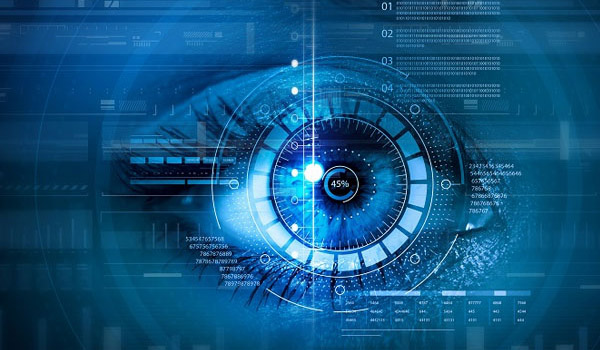
\includegraphics[width=0.65\textwidth]{computer-vision-la-gi.jpg}
	\caption[Computer Vision.]{Computer Vision.}
	\label{fig:ML}
\end{figure} 

Tuy rằng công nghệ xử lý thông tin hình ảnh đã xuất hiện từ lâu nhưng phần lớn quy trình vẫn đòi hỏi sự can thiệp của con người, tốn nhiều thời giờ và dễ bị lỗi. Ví dụ: việc triển khai hệ thống nhận diện khuôn mặt trước đây yêu cầu nhà phát triển phải gắn thẻ thủ công hàng ngàn hình ảnh bằng các điểm dữ liệu chính, chẳng hạn như chiều rộng sống mũi và khoảng cách giữa hai mắt. Tự động hóa các tác vụ này đòi hỏi sức mạnh điện toán rộng lớn vì dữ liệu hình ảnh không có cấu trúc và phức tạp để máy tính có thể sắp xếp. Do đó, ứng dụng thị giác tốn kém và hầu hết các tổ chức không thể tiếp cận.

Ngày nay, tiến bộ trong lĩnh vực này kết hợp với sự tăng cường đáng kể của sức mạnh điện toán đã cải thiện cả quy mô và độ chính xác của quy trình xử lý dữ liệu hình ảnh. Các hệ thống thị giác máy tính được hỗ trợ bởi tài nguyên điện toán đám mây hiện giờ trở nên dễ tiếp cận với tất cả mọi người. Bất kỳ tổ chức nào cũng có thể sử dụng công nghệ này để xác minh danh tính, kiểm duyệt nội dung, phân tích video phát trực tuyến, phát hiện lỗi và nhiều tính năng khác.

\section{Các trường hợp sử dụng của thị giác máy tính là gì?}
Nhiều ứng dụng thị giác máy tính được sử dụng trong lĩnh vực giải trí, kinh doanh, chăm sóc sức khỏe, giao thông vận tải và cuộc sống hàng ngày. Hãy cùng xem xét một số trường hợp sử dụng dưới đây:
\begin{itemize}
	\item Bảo mật và an toàn
	
	\item Hiệu quả hoạt động

	
	\item Chăm sóc sức khỏe
 
        \item Phương tiện tự hành
        

\end{itemize}

\section{Human Activity Recognition là gì? }

Human Activity Recognition (HAR) là một nhánh của ngành khoa học máy tính, với mục tiêu là tạo ra các hệ thống và kỹ thuật có khả năng tự động nhận dạng và phân loại các hành động của con người dựa trên dữ liệu cảm biến. HAR sử dụng các cảm biến để giải thích các cử chỉ hoặc chuyển động của cơ thể con người và xác định hoạt động hoặc chuyển động của con người.

Các hệ thống HAR thường được sử dụng trong nhiều ứng dụng khác nhau, bao gồm chăm sóc sức khỏe, vận động, an ninh, biểu diễn thể thao, v.v.

Trong khi xây dựng mô hình, mục tiêu của hệ thống HAR là dự báo nhãn hành động của một người trong hình ảnh hoặc video, thường được thực hiện thông qua nhận dạng hoạt động dựa trên video và nhận dạng hoạt động dựa trên hình ảnh.
\newpage

\section{HAR hoạt động như thế nào?} 

\begin{figure}[h!]
	\centering
	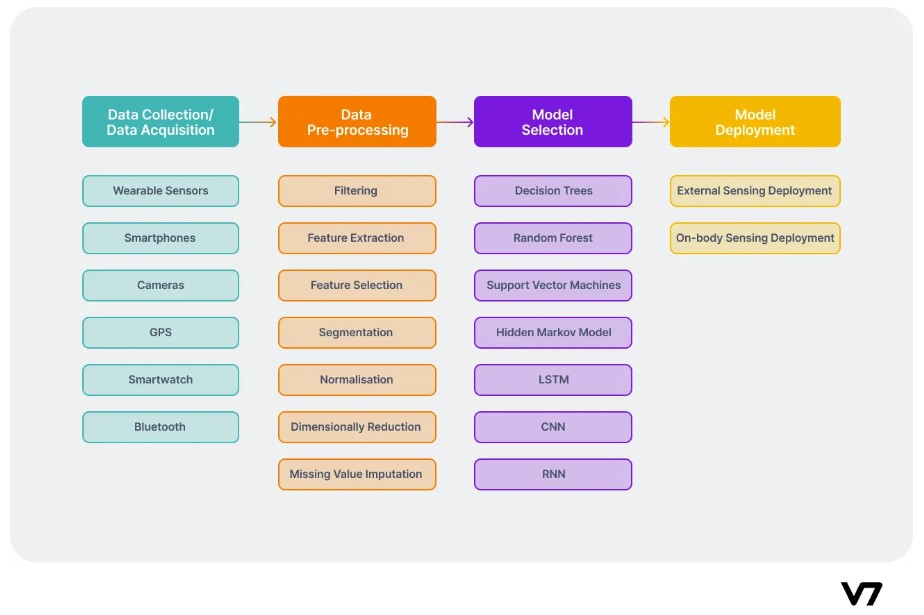
\includegraphics[width=0.65\textwidth]{Figures/flowchart.jpg}
	\caption[Flow Chart.]{Flow Chart.}
	\label{fig:ML}
\end{figure} 

\subsection{Mô tả bài toán thực tế} 

\begin{itemize}
	\item Sử dụng mạng CNN và LSTM để huấn luyện một mô hình có thể nhận biết hành động dựa vào webcam hoặc video  
	
	\item Đưa hành động vào webcam hoặc video chứa hành hành động vào model để dự đoán 

\end{itemize}

\subsection{Hướng tiếp cận bài toán }

\begin{itemize}
	\item Sử dụng thư viện MediaPipe và mạng LSTM với đầu vào là hành động trước webcam và đầu ra là phân loại hành động đó
	
	\item Sử dụng lớp layer ConvLSTM 
        \item Xây dựng mô hình LRCN
 

\end{itemize}

